%==================================================================================
%  articulo_smartcitynetV4.tex  ---  SmartCityNet, Version 4 (English, B1--B2)
%
%  "A Web Platform for Generating Optimization-Ready V2V/V2I Connectivity Data
%   from SUMO Vehicular Scenarios"
%
%  V4 = V3 + revisión aplicada (verde \revdel eliminado, azul \revadd aceptado a
%  texto normal) + rojos resueltos con datos REALES corridos sobre la red de Quito.
%  Cambio de fondo: el "grado" es ahora el número de VECINOS ÚNICOS (grafo no
%  dirigido), por lo que A--D y las métricas de conectividad se regeneraron.
%----------------------------------------------------------------------------------
%  >>> NECESITAS la carpeta Definitions/ y fig_rsu_map.pdf junto a este .tex. <<<
%  Rojo \todo{} = tarea/dato que solo el autor puede cerrar (citas §2, funding, repo).
%==================================================================================
\documentclass[engproc,proceedingpaper,submit,oneauthor]{Definitions/mdpi}

%------------------------------ MDPI internal (no modificar) -----------------------
\firstpage{1}
\makeatletter
\setcounter{page}{\@firstpage}
\makeatother
\pubvolume{1}
\issuenum{1}
\articlenumber{0}
\pubyear{2026}
\copyrightyear{2026}
\datereceived{ }
\dateaccepted{ }
\datepublished{ }

%============================== Paquetes adicionales ===============================
\usepackage[ruled,vlined,linesnumbered]{algorithm2e}
\usetikzlibrary{arrows.meta,positioning,shapes.geometric,calc,fit,backgrounds}

% ---- Colores y marca de pendiente (solo tareas de autor) ----
\definecolor{todored}{RGB}{185,0,0}
\definecolor{softgray}{RGB}{246,247,249}
\DeclareRobustCommand{\todo}[1]{{\color{todored}\textbf{[TO DO: #1]}}}

% ---- Atajos matemáticos ----
\newcommand{\Atil}{\widetilde{A}}
\newcommand{\bin}[1]{\beta\!\left(#1\right)}
\newcommand{\nnz}{\operatorname{nnz}}
\newcommand{\CVR}{\mathrm{CVR}}

%============================== Portada / metadatos ================================
\Title{A Web Platform for Generating Optimization-Ready V2V/V2I Connectivity Data
from SUMO Vehicular Scenarios}

\newcommand{\orcidauthorA}{0000-0000-0000-000X}

\Author{Edison Xavier Espinel Sevilla $^{1,}$*\orcidA{}}

\AuthorNames{Edison Xavier Espinel Sevilla}

\address{%
$^{1}$ \quad Escuela Politécnica Nacional, Quito, Ecuador; edison.espinel@epn.edu.ec}

\corres{Correspondence: edison.espinel@epn.edu.ec}

% Abstract (sin líneas en blanco). En la clase MDPI \abstract es un COMANDO.
\abstract{Roadside-unit (RSU) deployment models need data that tell which vehicles
can reach each candidate RSU, in which mobility snapshot, and with how many hops.
Producing these data is not trivial: it means combining traffic mobility, urban
geometry, direct-link evaluation, graph processing, and optimization-oriented data
structures. This paper presents a web platform that turns a geographical area and a
SUMO mobility scenario into an optimization-ready connectivity dataset. The backend
integrates OpenStreetMap and SUMO tools, filters candidate RSU positions, evaluates
binary V2V and V2I links from communication range and building obstruction, and
computes cumulative and minimum-hop connectivity through a matrix recurrence. A formal
proposition justifies the recurrence used by the pipeline: it recovers every
vehicle--RSU relation within a given hop limit, while first-arrival matrices identify
the minimum hop count. A Streamlit frontend supports configuration, execution,
visualization, and export. On the Historic Centre of Quito, varying the minimum
junction degree and the clustering radius keeps between 14 and 393 of 1211 eligible
junctions as candidates (about 68\% to 99\% reduction). The workflow separates mobility
simulation from infrastructure optimization, so the same dataset can feed different
exact or heuristic deployment models.}

\keyword{VANET; V2V connectivity; V2I connectivity; SUMO; multi-hop connectivity;
roadside units; preprocessing; facility location; operations research}

%==================================================================================
\begin{document}

%----------------------------------------------------------------------------------
\section{Introduction}

Vehicular ad hoc networks (VANETs) enable direct vehicle-to-vehicle (V2V)
communication and vehicle-to-infrastructure (V2I) communication with fixed roadside
units (RSUs), usually installed at intersections. Where these units are placed affects
coverage, path length, infrastructure cost, and network performance, so RSU deployment
is often stated as a facility-location problem and solved with exact, heuristic, or
metaheuristic methods.

These models need connectivity information \emph{before} the optimization starts:
which vehicles can reach each candidate RSU in each snapshot, and the minimum number of
relay hops. Producing it is not a minor step, as it combines traffic simulation,
vehicle-position extraction, urban geometry, range checks, obstacle detection, graph
processing, and conversion into the structures a solver accepts. Yet many deployment
studies treat these data as already available. The software side is similar: SUMO and
Python libraries are usually glued together with ad-hoc scripts, which hurts
reproducibility and reuse across formulations.

This work fills that gap with a web-based preprocessing layer that follows the
sequence
\[
\begin{aligned}
\text{urban area}\rightarrow{}&\text{SUMO snapshots}\rightarrow\text{candidate RSUs}
\rightarrow\text{V2V/V2I matrices}\\
&\rightarrow\text{minimum-hop tuples}\rightarrow\text{optimization input}.
\end{aligned}
\]
Its main output is not just a set of connectivity matrices, but a traceable dataset
that keeps the relation between geographical positions, SUMO identifiers, matrix
indices, snapshots, hop counts, and optimization identifiers. The contributions are:
(i)~a web platform that integrates a Streamlit frontend with a Python/SUMO backend in a
reproducible workflow; (ii)~automatic generation of direct V2V and V2I matrices under a
binary communication-range and line-of-sight (LoS) model; (iii)~a configurable
two-stage method that reduces the candidate RSU set using junction degree and spatial
clustering; (iv)~computation of cumulative and minimum-hop vehicle--RSU matrices;
(v)~export of optimization-ready dense structures and sparse tuples, including an
artificial no-service option per vehicle; (vi)~a formal justification of the recurrence
and minimum-hop representation used in the data-generation pipeline; and (vii)~a
sensitivity analysis of how the minimum degree and clustering radius change the number
of retained candidates. The optimization model that picks the final deployment is out
of scope: the goal is to generate its input automatically and independently of any
formulation.

%----------------------------------------------------------------------------------
\section{Related Work}\label{sec:related}

\subsection{RSU Deployment and Facility-Location Models}
RSU deployment has been studied through covering, median, routing, and stochastic
formulations. Maximal-covering models try to cover the largest demand with a limited
number of RSUs; set-covering models minimize how many units are needed to satisfy
coverage; and median-type models reduce the average distance or hop count.
Mobility-aware formulations extend these ideas over several traffic snapshots. The
stochastic model in~\citep{ref-urquiza} uses scenario-dependent connectivity tuples
and adds an artificial disconnected RSU as a no-service alternative that keeps the
problem feasible when a vehicle cannot, or should not, be assigned to a deployed real
RSU.

Despite their differences, all of these formulations rely on a common data layer:
candidate RSUs, vehicle sets, mobility scenarios, and feasible vehicle--RSU
relationships. This work focuses on producing exactly that layer. \todo{Complete
this subsection with recent studies on mobility-aware RSU placement, multi-hop
access, and exact or heuristic deployment. Every added reference must be cited in the
text.}

\subsection{SUMO-Based Platforms and Web Interfaces}
SUMO is an open-source microscopic traffic simulator with utilities to import OSM
networks, generate vehicle trips, run simulations, and export floating-car data
(FCD)~\citep{ref-sumo,ref-osm}. Streamlit and Folium support interactive Python web
interfaces and geographical visualization~\citep{ref-streamlit,ref-folium}. Their
individual capabilities are not, by themselves, the contribution of this work. The
contribution is their orchestration together with candidate filtering, geometric
direct-link evaluation, multi-hop processing, identifier traceability, and export to
optimization models.

Existing SUMO-based applications often focus on simulation control or visualization.
This platform instead treats simulation as the first stage of a data-generation
process whose final output can be consumed by facility-location and network-design
formulations. \todo{Add a short comparison with the closest scientific platforms,
considering mobility simulation, obstacle-aware V2V/V2I generation, multi-hop
processing, web interaction, optimization export, and reproducibility.}

%----------------------------------------------------------------------------------
\section{Web Platform and Connectivity-Data Generation}\label{sec:method}

\subsection{Platform Architecture and Workflow}
The platform follows a simplified model--view--controller organization. The Streamlit
frontend captures the area and the parameters, launches the workflow, and displays
maps, matrices, and summary indicators, while the Python backend prepares the SUMO
scenario, extracts snapshots, filters candidate RSUs, evaluates direct links, computes
multi-hop reachability, and exports the dataset; an orchestrator coordinates the
modules and stores each run's configuration. As shown in
Figure~\ref{fig:architecture}, OSM data become a SUMO network and building polygons
through \texttt{netconvert} and \texttt{polyconvert}, \texttt{randomTrips.py} generates
the demand, and the simulation produces the FCD snapshots that feed the connectivity
engine.

\begin{figure}[H]
\centering
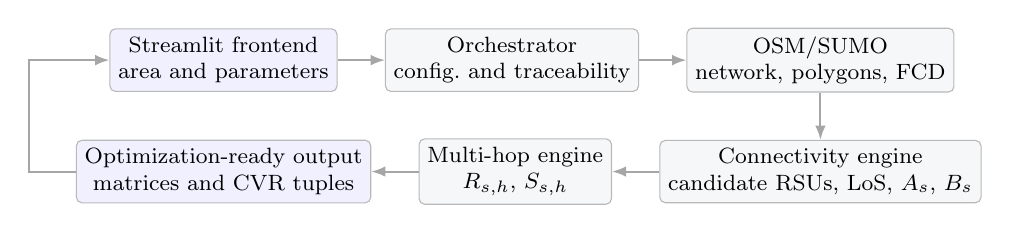
\begin{tikzpicture}[
  font=\footnotesize,
  box/.style={draw=gray!55,rounded corners=2pt,align=center,inner sep=3pt,
              minimum height=6mm,fill=softgray},
  main/.style={box,fill=blue!6},
  arr/.style={draw=gray!70,line width=.7pt,-{Latex[length=1.8mm]}}
]
\node[main] (ui) {Streamlit frontend\\area and parameters};
\node[box,right=6mm of ui] (orc) {Orchestrator\\config.\ and traceability};
\node[box,right=6mm of orc] (sumo) {OSM/SUMO\\network, polygons, FCD};
\node[box,below=6mm of sumo] (links) {Connectivity engine\\candidate RSUs, LoS, $A_s$, $B_s$};
\node[box,left=6mm of links] (hop) {Multi-hop engine\\$R_{s,h}$, $S_{s,h}$};
\node[main,left=6mm of hop] (out) {Optimization-ready output\\matrices and $\CVR$ tuples};
\draw[arr] (ui)--(orc); \draw[arr] (orc)--(sumo); \draw[arr] (sumo)--(links);
\draw[arr] (links)--(hop); \draw[arr] (hop)--(out);
\draw[arr] (out.west) -- ++(-6mm,0) |- (ui.west);
\end{tikzpicture}
\caption{Platform architecture and end-to-end data-generation workflow.}
\label{fig:architecture}
\end{figure}

The configurable parameters are grouped into mobility settings (bounding box,
simulation duration, vehicle generation, snapshot interval, and random seed),
candidate-selection settings (minimum junction degree $g_{\min}$ and clustering radius
$\rho$), communication settings (V2V/V2I range and building obstruction), and the
maximum hop count $H$. In the case study the interface used a V2V/V2I range of
$300$~m, a $120$~s snapshot interval, $g_{\min}=4$, and $\rho=20$~m as defaults.

\subsection{Candidate RSU Selection}
SUMO can produce a large set of junctions, including intermediate road points,
internal nodes, and closely located intersections; using all of them as candidates
enlarges the search space and adds nearly equivalent positions. The platform therefore
applies a two-stage reduction. First, directed and parallel SUMO edges are reduced to
unique unordered pairs of non-internal junctions; the degree of a junction is therefore
the number of distinct neighboring junctions in this undirected simple graph. Nodes
with degree below $g_{\min}$ are discarded. Second, the survivors are ordered by
decreasing degree and, when degrees are equal, by increasing SUMO junction identifier.
Greedy spatial clustering then accepts a node only if its distance to every previously
accepted candidate exceeds $\rho$. Coordinates are projected to UTM zone~17S before
clustering, so $\rho$ and all pairwise distances are measured in metres. Because
higher-degree nodes are processed first, they represent their local groups, while the
identifier tie-break makes repeated runs deterministic.

\begin{algorithm}[H]
\caption{Candidate RSU filtering by degree and greedy spatial clustering}
\label{alg:candidates}
\KwIn{Junction set $J$, unique unordered junction-pair set $E_u$, minimum degree
$g_{\min}$, clustering radius $\rho$ in projected metres}
\KwOut{Candidate RSU set $C$}
Initialize $\deg(j)\leftarrow 0$ for all $j\in J$\;
\ForEach{$\{u,v\}\in E_u$}{increment $\deg(u)$ and $\deg(v)$\;}
$F\leftarrow\{\,j\in J:\deg(j)\ge g_{\min}\,\}$\;
Sort $F$ by non-increasing degree and then by increasing SUMO identifier\;
$C\leftarrow\emptyset$\;
\ForEach{$j\in F$}{
  \If{$C=\emptyset$ \textbf{or} $\min_{c\in C}\operatorname{dist}(j,c)>\rho$}{
    $C\leftarrow C\cup\{j\}$\;
  }
}
\Return{$C$}\;
\end{algorithm}

This is a preprocessing heuristic, not an optimal RSU-placement algorithm. Its purpose
is to build a manageable candidate set before the deployment model is solved. Since it
may drop a location that would later be useful, the sensitivity of the retained set to
$(g_{\min},\rho)$ is reported in Section~\ref{sec:results} instead of hiding these
choices as fixed constants.

\subsection{Direct and Multi-Hop Connectivity}
For each snapshot $s\in\mathcal S$, let $\mathcal V_s=\{v_1,\ldots,v_{n_s}\}$ be the
active vehicles and $\mathcal R=\{r_1,\ldots,r_m\}$ the candidate RSUs. The binary V2V
matrix $A_s\in\{0,1\}^{n_s\times n_s}$ has $(A_s)_{ij}=1$ when $v_i$ and $v_j$ are
within the V2V range and no building polygon blocks the segment joining them; under the
bidirectional-link model it is symmetric. The binary V2I matrix
$B_s\in\{0,1\}^{n_s\times m}$ has $(B_s)_{ik}=1$ when $v_i$ can directly reach $r_k$
under the V2I range and LoS. Obstruction uses a 2-D segment--polygon intersection test,
so the result is a geometric binary approximation; it does not model attenuation,
fading, interference, or packet delivery.

A vehicle without direct V2I access may still reach an RSU through other vehicles.
Define the augmented adjacency matrix $\Atil_s=\bin{A_s+I}$, where $\beta(X)$ maps
every positive entry of $X$ to one and every zero entry to zero. Cumulative
connectivity is
\begin{align}
R_{s,1} = B_s,\qquad
R_{s,h} = \bin{\Atil_s R_{s,h-1}},\quad h=2,\ldots,H.\label{eq:rh}
\end{align}
The identity term keeps the paths already found at smaller hop counts, which gives
$R_{s,1}\le R_{s,2}\le\cdots\le R_{s,H}$ elementwise. The first-arrival matrices are
$S_{s,1}=R_{s,1}$ and $S_{s,h}=R_{s,h}-R_{s,h-1}$ for $h\ge 2$.

\begin{Proposition}\label{prop:reachability}
For any snapshot $s$, $(R_{s,h})_{ik}=1$ if and only if there is a path from vehicle
$v_i$ to candidate RSU $r_k$ using at most $h$ communication hops, where the final hop
is V2I and every previous hop is V2V.
\end{Proposition}

\begin{proof}
By induction on $h$. For $h=1$, $R_{s,1}=B_s$, so an entry is one exactly for a direct
V2I link. Assume the statement holds for $h-1$. The entry $(\Atil_s R_{s,h-1})_{ik}$
is positive if there is an index $j$ with $(\Atil_s)_{ij}=1$ and $(R_{s,h-1})_{jk}=1$.
If $j=i$, the identity term keeps a path of at most $h-1$ hops. If $j\neq i$, then
$(A_s)_{ij}=1$ adds one V2V hop from $v_i$ to $v_j$ before a path of at most $h-1$ hops
from $v_j$ to $r_k$. Conversely, every path of at most $h$ hops either already has at
most $h-1$ hops or begins with one V2V hop followed by such a path. Binarization
therefore gives exactly the stated reachability relation.
\end{proof}

\begin{Corollary}\label{cor:minhop}
For $h\ge 2$, $(S_{s,h})_{ik}=1$ if and only if the minimum number of hops from $v_i$
to $r_k$ is exactly $h$; for $h=1$, $S_{s,1}=B_s$ identifies the direct connections.
\end{Corollary}

The corollary follows from Proposition~\ref{prop:reachability} and the monotonicity of
$R_{s,h}$: each reachable vehicle--RSU pair appears for the first time at a single hop
value only. Figure~\ref{fig:matrices} shows a compact example. Under ordinary dense
matrix multiplication, each product of an $n_s\times n_s$ matrix by an $n_s\times m$
matrix costs $O(n_s^2m)$. Computing all levels therefore takes
$O((H-1)n_s^2m)=O(Hn_s^2m)$ time per snapshot, while retaining every cumulative or
first-arrival matrix requires $O(Hn_sm)$ space. Sparse matrices, bitsets, Boolean
algebra, or parallel kernels may improve actual runtimes, but they are not used to
weaken these dense worst-case bounds. The recurrence is presented as a formally
justified component of the preprocessing pipeline, not as a new graph-search algorithm.

\begin{figure}[H]
\centering
\newcommand{\hc}[1]{\ifnum#1=1\cellcolor{violet!60}\textcolor{white}{1}\else\cellcolor{gray!8}0\fi}
\small
\begin{tabular}{c@{\hskip 6mm}c@{\hskip 6mm}c}
\begin{tabular}{c|ccc}
$R_3$ & $r_1$ & $r_2$ & $r_3$\\\hline
$v_1$ & \hc1 & \hc1 & \hc1\\
$v_2$ & \hc1 & \hc1 & \hc1\\
$v_3$ & \hc1 & \hc1 & \hc1\\
$v_4$ & \hc0 & \hc0 & \hc0
\end{tabular}&
\begin{tabular}{c|ccc}
$S_2$ & $r_1$ & $r_2$ & $r_3$\\\hline
$v_1$ & \hc0 & \hc0 & \hc1\\
$v_2$ & \hc1 & \hc1 & \hc0\\
$v_3$ & \hc0 & \hc0 & \hc1\\
$v_4$ & \hc0 & \hc0 & \hc0
\end{tabular}&
\begin{tabular}{c|ccc}
$S_3$ & $r_1$ & $r_2$ & $r_3$\\\hline
$v_1$ & \hc0 & \hc1 & \hc0\\
$v_2$ & \hc0 & \hc0 & \hc0\\
$v_3$ & \hc1 & \hc0 & \hc0\\
$v_4$ & \hc0 & \hc0 & \hc0
\end{tabular}
\end{tabular}
\caption{Illustrative cumulative ($R_3$) and first-arrival ($S_2$, $S_3$) matrices for
$H=3$. Purple cells in $R_3$ indicate reachability within at most three hops, whereas
purple cells in $S_2$ and $S_3$ identify first arrivals at exactly two and three hops,
respectively. Vehicle $v_4$ reaches no real RSU within the hop limit.}\label{fig:matrices}
\end{figure}

\subsection{Optimization-Oriented Export and Cardinality}
Let $K_s=\sum_{h=1}^{H}\nnz(S_{s,h})=\nnz(R_{s,H})$ be the number of reachable real
vehicle--RSU pairs in snapshot $s$. The export module creates one tuple for each real
pair at its minimum hop and one artificial no-service tuple for every active vehicle:
\[
\CVR_s=
\{\langle s,h,i,k\rangle:(S_{s,h})_{ik}=1\}
\cup
\{\langle s,H+1,i,r_\infty\rangle:i\in\mathcal V_s\}.
\]
The artificial RSU $r_\infty$ (identifier $0$) is not only physical disconnection: it
is the optimization option of leaving a vehicle unserved when real candidates are not
deployed, are saturated, or are rejected by cost or capacity constraints. It is
therefore included even when the vehicle can reach real RSUs, and is penalized at hop
$H+1$. The cardinality is $|\CVR_s|=K_s+n_s$, with $n_s\le|\CVR_s|\le n_s(m+1)$ for
$m\ge 1$; the hop limit $H$ does not multiply the real tuples, since each reachable
pair is exported once, at its minimum hop. The dataset can be written to an
OPL/\texttt{.dat} file or kept in memory for other solvers.

Across all snapshots, define
\[
N=\sum_{s\in\mathcal S}n_s,\qquad
K=\sum_{s\in\mathcal S}\nnz(R_{s,H}),\qquad
|\CVR|=K+N.
\]
Here $N$ counts vehicle--snapshot instances rather than distinct vehicle identifiers.
Consequently, a valid export must contain exactly $K$ real tuples and exactly $N$
artificial tuples. This identity provides a direct integrity check for the generated
dataset.

%----------------------------------------------------------------------------------
\section{Experimental Results}\label{sec:results}

\subsection{Experimental Settings}
The evaluation uses one real scenario in the Historic Centre of Quito, Ecuador. The
goal is not to compare cities but to measure how the candidate-generation parameters
change the size of the optimization search space while the road network stays fixed.
The two factors are the minimum junction degree $g_{\min}$ and the greedy clustering
radius $\rho$. The imported network has $1211$ eligible junctions; the SUMO run covered
$0$--$3660$~s and, sampled every $120$~s, produced $31$ snapshots. The scenario
involves $132$ distinct vehicle identifiers over the complete run; the number of
\emph{active} vehicles per snapshot ranges from $1$ to $9$ (mean $6.5$), giving a
vehicle--snapshot total $N=\sum_s n_s=201$. Both direct V2V and V2I ranges were
$300$~m, and the maximum hop count was $H=3$. All configurations reuse the same network
and node-exclusion rule, which isolates the effect of $(g_{\min},\rho)$. The study area
(Figure~\ref{fig:rsumap}) corresponds to an OpenStreetMap extract spanning about
$-78.535^{\circ}$ to $-78.497^{\circ}$ longitude and $-0.266^{\circ}$ to
$-0.211^{\circ}$ latitude (UTM zone~17S, WGS84), downloaded on 5~June~2026. The pipeline
ran with SUMO~1.26.0 and Python~3.10 (NumPy~2.2, pandas~2.3) on an AMD~Ryzen~7~7735HS
(8~cores/16~threads) with $16$~GB RAM under Windows~11 (x86-64). Vehicle demand was
generated with \texttt{randomTrips.py} (\texttt{-e 3660}, inserting the $132$ trips
over the horizon, mean headway~$\approx28$~s) using its default seed (no
\texttt{-{}-random} flag), so the mobility can be reproduced provided that the remaining
generation parameters are fixed.

\subsection{Results}
Table~\ref{tab:sensitivity} reports, for four configurations, the count after degree
filtering $|F|$, the retained candidates $Y$, and the reduction $100(1-Y/X)$ over the
$X=1211$ eligible junctions. The retained count decreased across the tested
configurations. Comparison A--B isolates the increase in $\rho$ at $g_{\min}=3$,
whereas B--C isolates the increase in $g_{\min}$ at $\rho=20$~m; C--D changes both
factors and therefore does not identify either effect separately. These four runs
provide a limited sensitivity check rather than a global monotonicity result for the
greedy procedure. The permissive setting~(A) keeps $393$ candidates ($67.5\%$
reduction), while the restrictive setting~(D) keeps only $14$ ($98.8\%$): in this
grid-like centre very few junctions have five or more distinct street neighbours, so
$g_{\min}=5$ is highly selective. The reference setting~(C, $g_{\min}=4$,
$\rho=20$~m) retains $278$ candidates, about a quarter of the eligible junctions;
Figure~\ref{fig:rsumap} maps these candidates over the study area.

\begin{table}[H]
\centering
\caption{Candidate-set sensitivity in the Historic Centre of Quito
($X=1211$ eligible junctions). Values were produced by running the corrected filtering
code (undirected unique-neighbour degree) on the same network.}\label{tab:sensitivity}
\small
\begin{tabular}{cccccc}
\toprule
Config. & $g_{\min}$ & $\rho$ (m) & After degree $|F|$ &
Candidates $Y=|C|$ & Reduction (\%)\\
\midrule
A & 3 & 15 & 1097 & 393 & 67.5\\
B & 3 & 20 & 1097 & 366 & 69.8\\
C & 4 & 20 & \phantom{0}836 & 278 & 77.0\\
D & 5 & 25 & \phantom{00}15 & \phantom{0}14 & 98.8\\
\bottomrule
\end{tabular}
\end{table}

Rows A and B share $|F|=1097$ because they use the same $g_{\min}=3$, so their
difference isolates the clustering radius; the extra drop from B to C ($|F|$ from
$1097$ to $836$) is the effect of the stricter degree threshold before clustering.

This matters because binary deployment variables and many assignment or routing
structures grow with the number of candidate facilities. A smaller set is not
automatically better, though: it speeds up the model but may drop useful locations, so
the reduction is a preprocessing trade-off, not proof of a better deployment. For the
reference configuration, the platform completed the full transformation from snapshots
to matrices and tuples; Table~\ref{tab:multihop-cvr} reports the verified connectivity
and export metrics, all computed from the same run and satisfying the integrity
identity $|\CVR|-K=N$.

\begin{table}[H]
\centering
\caption{Connectivity and export metrics for the reference configuration
(C, $g_{\min}=4$, $\rho=20$~m, $278$ candidate RSUs, $H=3$), computed from the same
run.}\label{tab:multihop-cvr}
\footnotesize
\begin{tabular}{p{0.25\linewidth}p{0.52\linewidth}p{0.10\linewidth}}
\toprule
Metric & Calculation and meaning & Result\\
\midrule
Hop limit & Maximum number of communication hops, including the final V2I hop & $H=3$\\
Direct real pairs & $M_1=\sum_s\nnz(S_{s,1})$ & $1310$\\
New real pairs by hop & $M_2=\sum_s\nnz(S_{s,2})$; \; $M_3=\sum_s\nnz(S_{s,3})$ &
$109$; $8$\\
All reachable real pairs & $K=\sum_{h=1}^{H}M_h=\sum_s\nnz(R_{s,H})$ & $1427$\\
Vehicle--snapshot instances & $N=\sum_s n_s$; not the number of distinct vehicle
identifiers ($132$) & $201$\\
Exported tuple set & $|\CVR|=K+N$; $K$ real tuples plus one artificial tuple per
vehicle--snapshot instance & $1628$\\
Runtime and output size & Direct-link construction $\approx4.0$~s; multi-hop
computation $<0.1$~s; export; final \texttt{.dat} size & $63$~KB\\
\bottomrule
\end{tabular}
\end{table}

The sequence $M_h$ measures the marginal reachability obtained at each additional hop,
while $K$ is cumulative; here multi-hop forwarding adds only $M_2+M_3=117$ pairs beyond
the $1310$ direct ones, because with a mean of $6.5$ active vehicles per snapshot there
are few relays available. The equality $|\CVR|-K=N$ holds exactly ($1628-1427=201$);
otherwise, some artificial tuples would be missing or duplicated. Table~\ref{tab:excerpt}
shows a verified export excerpt with three real tuples at increasing minimum hop and one
artificial tuple, together with the mappings from optimization identifiers back to
snapshot time and SUMO identifiers.

\begin{table}[H]
\centering
\caption{Verified export excerpt (reference configuration). Optimization identifiers
$\langle s,h,i,k\rangle$ and their mapping to snapshot time, SUMO vehicle, and SUMO
junction.}\label{tab:excerpt}
\small
\begin{tabular}{lllll}
\toprule
$\langle s,h,i,k\rangle$ & Meaning & Snapshot $t$ (s) & SUMO vehicle & SUMO junction\\
\midrule
$\langle 1,1,0,22\rangle$ & direct (1 hop) & $0$ & V0 & 11135269234\\
$\langle 4,2,13,46\rangle$ & 2 hops & $360$ & V13 & 267037290\\
$\langle 26,3,116,50\rangle$ & 3 hops & $3000$ & V116 & 268253365\\
$\langle 1,4,0,0\rangle$ & artificial ($r_\infty$) & $0$ & V0 & --- (no service)\\
\bottomrule
\end{tabular}
\end{table}

\begin{figure}[H]
\centering
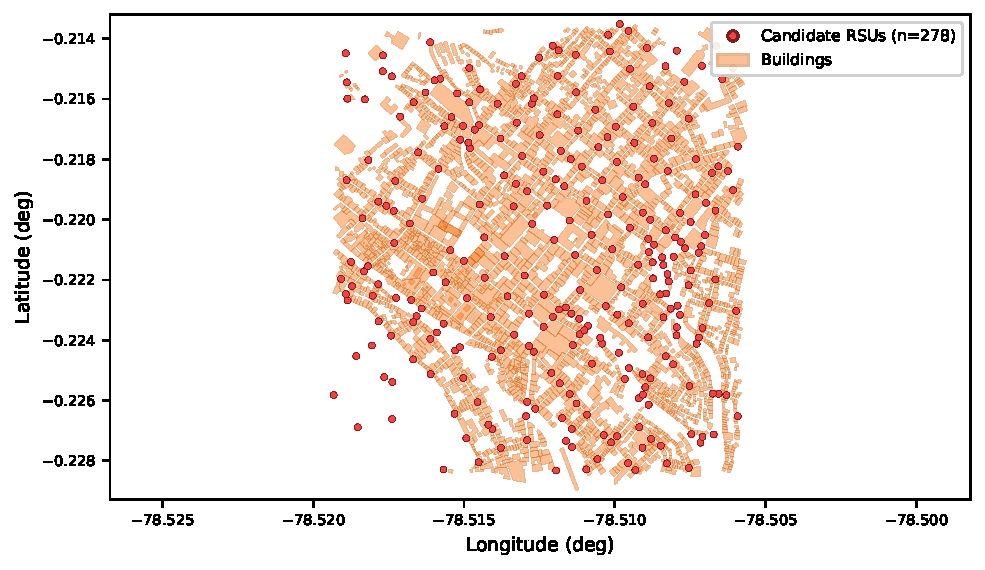
\includegraphics[width=0.6\linewidth]{fig_rsu_map.pdf}
\caption{Candidate RSUs produced by the platform for the reference configuration
(C, $g_{\min}=4$, $\rho=20$~m; $n=278$, red) over the building footprints (orange) of
the Historic Centre of Quito, in geographical coordinates.}\label{fig:rsumap}
\end{figure}

The main limitations are as follows: the binary geometric link model uses 2-D building
footprints without height and ignores path loss, fading, interference, channel load,
and packet reliability; each snapshot is processed independently, so the recurrence
describes paths \emph{inside} a snapshot, not time-respecting store-carry-forward
routes, and it does not include relay latency; candidate filtering is heuristic, with
its effect on a later deployment objective still unquantified; and the quality of the
final deployment depends on the optimization model that consumes the generated data.

%----------------------------------------------------------------------------------
\section{Conclusions and Future Work}\label{sec:conclusions}

This paper presented a web platform that turns a geographical area and SUMO mobility
output into optimization-ready V2V/V2I connectivity data, combining candidate RSU
generation, direct-link evaluation with building obstruction, cumulative and
minimum-hop matrix processing, traceable identifiers, and export. A formal result
justifies the recurrence used by the pipeline: it recovers each vehicle--RSU relation
reachable within the hop limit, and the first-arrival matrices assign each real pair
its minimum hop; the exported set adds one artificial no-service option per vehicle, an
optimization decision rather than mere disconnection. On the Historic Centre of Quito,
filtering keeps $14$--$393$ of $1211$ eligible junctions depending on
$(g_{\min},\rho)$, a preprocessing trade-off that shrinks the model without
guaranteeing a better deployment. Future work includes comparing the recurrence against
breadth-first search, sparse and Boolean-semiring kernels, dynamic tuple generation
inside the optimization method (e.g.\ decomposition or column generation), richer
propagation and reliability models, and measuring the effect of filtering on deployment
cost, coverage, capacity, and solution time.

%----------------------------------------------------------------------------------
\authorcontributions{Conceptualization, methodology, software, validation,
writing---original draft preparation, and writing---review and editing, E.X.E.S. The
author has read and agreed to the published version of the manuscript.}

\funding{\todo{Confirm whether the work received institutional or project support
through SmartCityNet (e.g.\ PIGR-24-02). If applicable, insert the exact funder name,
project title/code, and grant information required by the venue; otherwise state
``This research received no external funding.''}}

\dataavailability{The source code and generated datasets (SUMO network, snapshots,
matrices, and exported tuples) will be made available from
\todo{insert the verified public or anonymized repository URL/DOI; if access is
restricted during review, state the access procedure}.}

\acknowledgments{During the preparation of this manuscript, an AI-based assistant was
used for LaTeX formatting and draft editing; the author reviewed and edited the content
and takes full responsibility for the publication.}

\conflictsofinterest{The author declares no conflict of interest.}

%----------------------------------------------------------------------------------
\reftitle{References}

\begin{thebibliography}{999}
\bibitem{ref-urquiza}
Urquiza-Aguiar, L.; Tripp-Barba, C.; Aguilar-Igartua, M. A Stochastic Optimization
Model for the Placement of Road Side Units. In {\em Proceedings of ADHOC-NOW};
Springer: Cham, Switzerland, 2016.

\bibitem{ref-sumo}
Lopez, P.A.; Behrisch, M.; Bieker-Walz, L.; et~al. Microscopic Traffic Simulation
using SUMO. In {\em Proceedings of the 21st IEEE International Conference on
Intelligent Transportation Systems}; IEEE: Maui, HI, USA, 2018; pp. 2575--2582.

\bibitem{ref-osm}
OpenStreetMap contributors. OpenStreetMap. Available online:
\url{https://www.openstreetmap.org} (accessed on 20 July 2026).

\bibitem{ref-streamlit}
Streamlit Inc. Streamlit. Available online: \url{https://streamlit.io} (accessed on
20 July 2026).

\bibitem{ref-folium}
Python Visualization. Folium: Python Data, Leaflet.js Maps. Available online:
\url{https://python-visualization.github.io/folium/} (accessed on 20 July 2026).
\end{thebibliography}

\PublishersNote{}
\end{document}
